
\item $504$ cones, each of diameter $3.5$ cm and height $3$ cm, are melted and recast into a metallic sphere. Find the diameter of the sphere and hence find its surface area.$\sbrak {use \pi = \frac{22}{7} }$

       \item The diagonal of a rectangular field is $16$ metres more than the shorter side. If the longer side is $14$ metres more than the shorter side, then find the lengths of the sides of the field.

        \item Due to sudden floods, some welfare associations jointly requested the government to get 100 tents fixed immediately and offered to contribute 50 of the cost. If the lower part of each tent is of the form of a cylinder of  diameter  $4.2$  m  and  height  $4$  m  with  the  conical  upper  part  of same diameter but of height $2.8$ m, and the canvas to be used costs \rupee~$100$ per sq. m, find the amount, the associations will have to pay. What values are shown by these associations ?$\sbrak {use \pi  = \frac{22}{7}}$

         \item A hemispherical bowl of internal diameter $36$ cm contains liquid. This liquid is filled into $72$ cylindrical bottles of diameter $6$ cm. Find the height of the each bottle, if $10\%$  liquid is wasted in this transfer.

         \item A cubical block of side $10$ cm is surmounted by a hemisphere. What is the largest diameter that the hemisphere can have ? Find the  cost  of painting the total surface area of the solid so formed, at the rate of  \rupee~$5$ per $100$ sq. cm.$ \sbrak { use \pi = 3.14}$
         \item In Figure $5$, $PQRS$ is a square lawn with side $PQ$ = $42$ metres.  Two circular flower beds are there on the sides $PS$ and $QR$ with centre at $O$, the intersection of its diagonals. Find the total area of the two flower beds $\brak{shaded parts}$
   \begin{figure}[h]
       \centering
       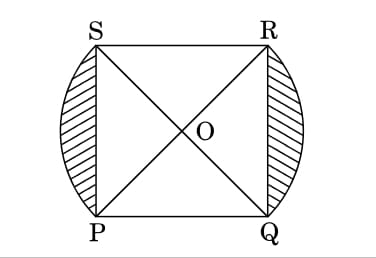
\includegraphics[width=0.5\linewidth]{figs/geo12.jpg}
    \end{figure}

       \item Find the area of the minor segment of a circle of radius $14$ cm, when its central angle is $60\degree$. Also find the area of the corresponding major segment.$\sbrak {use\pi= \frac{22}{7}}$
 \end{enumerate}
